%% -*- coding:utf-8 -*-

\chapter{空语类}
%\chapter{Empty elements}
\label{Abschnitt-Diskussion-leere-Elemente}
\label{chap-empty}

这一章介绍空语类,我们首先讨论不同研究传统对于空语类的总体态度,然后说明怎样能从语法中取消空语类(\ref{Abschnitt-Eleminierung-leerer-Elemente})。\ref{Abschnitt-leere-Elemente-Semantik}讨论为语义解释而设置的空语类。\ref{Abschnitt-Evidenz-leere-Elemente}主要从跨语言对比的角度讨论设置空语类的动因。\ref{Abschnitt-leere-Elemente-LRs-Transformations}介绍一些有关转换、词汇规则和空语类可以相互转换的观点。
%This chapter deals with empty elements, I first discuss the general attitude of various research
%traditions towards empty elements and then show how they can be eliminated from grammars
%(Section~\ref{Abschnitt-Eleminierung-leerer-Elemente}). Section~\ref{Abschnitt-leere-Elemente-Semantik} discusses empty elements that
%have been suggested in order to facilitate semantic
%interpretation. Section~\ref{Abschnitt-Evidenz-leere-Elemente} discusses possible motivation for
%empty elements with a special focus on cross-linguistic comparison and the final Section~\ref{Abschnitt-leere-Elemente-LRs-Transformations} shows
%that certain accounts with transformations, lexical rules, and empty elements can be translated into each other.

\section{有关空语类的观点}
%\section{Views on empty elements}

\isce[|(]{空成分}{empty element}特别具有争议的一个问题是是否需要设立空语类。关于空语类的讨论由来已久:在1961年已经有关于短语结构语法\isce{短语结构语法}{phrase structure grammar}的研究\citep*{BHPS61a}。关于空语类地位的讨论从那时候就开始了(例如,可以参见\citealp*{Loebner86a,Wunderlich87d,Wunderlich89,Stechow89,Haider97a,Sag2000a,BMS2001a,LH2006a,Mueller2004e,AS2015a})。有时候设立空语类和不设立空语类的分析还存在实际语料上的差异 \citep{AS2015a},但是通常情况下并不是这样。因为空语类经常用作证据来支持或反对某些理论,这里我们会更加详细地介绍它们是怎样被运用的。
%One\is{empty element|(} point that is particularly controversial among proponents of the theories discussed in this book is the question of whether
%one should assume empty elements or not.\todostefan{Add arguments from wanna contraction} The discussion of empty elements is quite old: there was already some investigation in 1961 with reference
%to phrase structure grammars\is{phrase structure grammar} \citep*{BHPS61a}.
%The discussion of the status of empty elements has carried on ever since (see
%\citealp*{Loebner86a,Wunderlich87d,Wunderlich89,Stechow89,Haider97a,Sag2000a,BMS2001a,LH2006a,Mueller2004e,AS2015a}, for example). 
%There are sometimes empirical differences between analyses that assume empty elements and those that
%do not \citep{AS2015a}, but often this is not the case. Since empty elements often feature prominently in the argumentation for or against particular theories, I will discuss
%how they have been used in somewhat more detail here.

在\gbtc 中,空语类用于解释移位遗留下来的语迹(动词移位和短语前置)以及省略\isce{省略}{ellipsis}构式中删除的成分。从 \citet{Larson88a}的分析开始,越来越多的空的中心语被引入用于确保句法结构以及一些语义解释的统一性\isce{统一性}{uniformity} (约束\isce{约束理论}{Binding Theory}和辖域\isce{辖域}{scope},见\ref{sec-little-v}对于\littlevc 的论述)。其他用于确保特定概括的空语类还有 \citet[\page 734]{Coopmans-89a-u}和 \citet[第1章]{Postal2004a-u}提出的虚位\iscesub{代词}{pronoun}{虚位}{expletive}。这些空语类填充了英语\ilce{英语}{English}中倒装\isce{倒装}{inversion}结构的主语位置,动词之前的位置被一个PP而不是一个明显的主语NP占据。与此相似, \citet[\page 1311]{Grewendorf93}认为无人称被动句\iscesub{被动}{passive}{无人称}{impersonal}和没有主语移位的被动句中的主语位置实际上都是由一个空的虚位所占据。也可以参见 \citew[\page 91]{Newmeyer2005a}和 \citet[\page 180]{Lohnstein2014a}采用同样假设对于德语被动句的分析。 \citet[第II.3.3.3节]{Sternefeld2006a-u}认为在例(\mex{1})中,无人称被动句和无主语句都有一个空的虚位。
%In \gbt, empty elements were assumed for traces of movement (verb movement and fronting of phrases) as well as for deleted elements in 
%elliptical\is{ellipsis} constructions. Starting with the analysis of  \citet{Larson88a}, more and more empty heads have been introduced to ensure uniformity\is{uniformity} of structures and 
%certain semantic interpretations (binding\is{Binding Theory}
%and s\textsc{cop}e\is{scope}, see Section~\ref{sec-little-v} on \littlev). Other examples of an empty element that was introduced in order to maintain particular generalizations are the empty expletives\is{pronoun!expletive}
%of  \citet[\page 734]{Coopmans-89a-u} and  \citet[Chapter~1]{Postal2004a-u}. These fill the subject
%position in inversion\is{inversion} structures in English\il{English}, where the position preceding
%the verb is occupied by a PP and not by an overt subject NP. Similarly,  \citet[\page
%  1311]{Grewendorf93} assumes that the subject position in impersonal
%passives\is{passive!impersonal} and passives without subject movement is in fact occupied by an
%empty expletive. Also, see
% \citew[\page 91]{Newmeyer2005a} and  \citet[\page 180]{Lohnstein2014a} for this assumption with regard to the passive
%in German.  \citet[Section~II.3.3.3]{Sternefeld2006a-u} assumes that there is an empty expletive subject in impersonal passives and subjectless sentences such as (\mex{1}).
\eal
\ex 
\gll Mir graut.\\
	 我.\dat{} 惊吓\\
\mytrans{我受到惊吓。}
%\gll Mir graut.\\
%	 me.\dat{} scares\\
%\mytrans{I am scared.}
\ex 
\gll Mich dürstet.\\
	我.\acc{} 渴\\
\mytrans{我渴。}
%\gll Mich dürstet.\\
%	 me.\acc{} is.thirsty\\
%\mytrans{I am thirsty.}
\zl

\noindent
在第\pageref{Beispiel-leeres-Element-intransitive-Verben}页,我们讨论了Stabler对于包含不及物动词句子的分析。因为,按照 \citet[\page 146]{Chomsky2008a},首先与中心语组合的是补足语,不及物动词对该理论提出了挑战。Stabler通过假设不及物动词与一个空宾语组合解决了这个问题\citep[\page 61,124]{Veenstra98a}。因为这些不发音的成分对某一表达的意义没有贡献,所以我们也将其处理为虚位代词。
%On page~\pageref{Beispiel-leeres-Element-intransitive-Verben}, we discussed Stabler's proposal for the analysis of sentences with intransitive
%verbs. Since, following   \citet[\page 146]{Chomsky2008a}, the element that first merges with a head is the complement, intransitive verbs pose a problem for the
%theory. This problem is solved by Stabler by assuming that intransitive verbs are combined with an empty object \citep[\page 61,
%124]{Veenstra98a}. Since these silent elements do not contribute to the meaning of an expression, we are also dealing with empty expletive pronouns.


在其他理论中,有人反对空语类,也有人赞成空语类。在范畴语法\indexcg 中,Steedman提出了一种不借助空语类的方式来分析非局部依存(见\ref{sce-nld-cg}),但是正如 \citet{Pollard88a}指出的那样,Steedman的分析需要为NP提供多种类型提升\isce{类型提升}{type raising}或者需要为关系代词\iscesub{代词}{pronoun}{关系}{relative}提供一个相应数量的复杂词项(见\ref{Abschnitt-CG-UDC})。而 \citet{KoenigE99a-u}却使用语迹进行了解释。在\ref{Abschnitt-GPSG-Fernabhaengigkeiten}中,我们曾经讨论过,在GPSG\indexgpsg 中, \citet[\page 76--77]{Uszkoreit87a}对于提取\isce{提取}{extraction}没有使用语迹进行分析,但是 \citet*[\page 143]{GKPS85a}的分析却使用了语迹。在LFG\indexlfg 中,同样有人用语迹\citep[\page 67]{Bresnan2001a},也有人不用(\ref{Abschnitt-Verbstellung-LFG}和\ref{Abschnitt-NLA-LFG})。HPSG\indexhpsg 中的很多短语分析都是为了避免使用空语类(见\ref{Abschnitt-Phrasale-Konstruktionen})。例如, \citet{Sag97a}对关系小句的分析,用相应的短语规则代替了 \citew{ps2}所用的空的关系化标记。但是, \citew{Bender2001a}和 \citew*[\page 464]{SWB2003a}却假设了一个空系词\isce{系词}{copula}。另外一个想要从HPSG中清除空语类的例子是用词库而不是语迹来描写长距离依存\citep*{BMS2001a}。但是,正如  \citet{LH2006a}所展示的,用词汇手段引入长距离依存的提取理论在处理并列结构的语义解释时是有问题的。关于如何解决这个问题,见 \citew{Chaves2009a}。有很多TAG分析\indextag 没有在词库中包含空语类,可参见\ref{TAG-Fernabh}和 \citew{Kroch87a},但是也有 \citet[\page 194]{Kallmeyer2005a-u}的TAG分析,假设一个语迹来给包含动词复杂结构的句子中的成分进行重新排序。 \citet[\page 10--11]{Rambow94a}假设每一个动词短语中都有一个空动词(见\ref{sec-vtag}对于V-TAG\iscesub{树邻接语法(TAG)}{Tree Adjoining Grammar (TAG)}{矢量树邻接语法(V-TAG)}{Vector (V-TAG)}的论述)。\dotfootnote{%
注意TAG中的空语类与其他理论中的空语类有细微差异。在TAG中,空语类通常是初级树的一部分,即它们不与其他成分组合。  
} 在依存语法中,\mel (\citeyear[\page 303]{Melcuk88a-u};\citeyear[\page 219]{Melcuk2003a-u})、 \citet[\page 253]{Starosta88a-u}、 \citet[\page 471--472]{Eroms2000a}、Hudson(\citeyear[第3.7节]{Hudson2007a-u}、\citeyear[\page 166]{Hudson2010b-u})和 \citet{Engel2014a}为限定语、名词、省略、祈使句、控制不定式和并列结构假设了空语类,但是 \citet[\page 73]{GO2009a}反对空语类(省略现象是例外,\citealp{Osborne2016a-u})。
%In other theories, there are researchers that reject empty elements as well as those who assume them.
%In Categorial Grammar\indexcg, Steedman suggests an analysis of nonlocal dependencies that does
%without empty elements (see Section~\ref{sce-nld-cg}), but as  \citet{Pollard88a} has shown,
%Steedman's analysis requires various kinds of type raising\is{type raising}
%for NPs or a correspondingly high number of complex lexical items for relative pronouns\is{pronoun!relative} (see Section~\ref{Abschnitt-CG-UDC}). On the other hand,
% \citet{Koenig99a-u} uses\todostefan{andere Quellen?}
%traces. In GPSG\indexgpsg, there is the trace-less analysis of extraction\is{extraction} by  \citet[\page 76--77]{Uszkoreit87a} that we discussed in 
%Section~\ref{Abschnitt-GPSG-Fernabhaengigkeiten}, but there is also the analysis of  \citet*[\page 143]{GKPS85a} that uses traces. In LFG\indexlfg, there are both analyses with
%traces \citep[\page 67]{Bresnan2001a} and those without (see Section~\ref{Abschnitt-Verbstellung-LFG} and Section~\ref{Abschnitt-NLA-LFG}). 
%Many of the phrasal analyses in HPSG\indexhpsg are born out of the wish to avoid empty elements (see Section~\ref{Abschnitt-Phrasale-Konstruktionen}). 
%An example for this is the relative clause analysis by  \citet{Sag97a} that replaces the empty
%relativizer in  \citew{ps2} with a corresponding phrasal rule. On the other hand we have
% \citew{Bender2001a} and  \citew*[\page 464]{SWB2003a}, who assume a silent \textsc{cop}ula\is{\textsc{cop}ula}. Another attempt to eliminate empty elements from HPSG was to handle
%long-distance dependencies not by traces but rather in the lexicon \citep*{BMS2001a}. As  \citet{LH2006a} could show, however, theories of extraction that
%introduce long-distance dependencies lexically have problems with the semantic interpretation of coordinate structures. For a suggestion of how to solve these problems,
%see  \citew{Chaves2009a}. There are many TAG analyses\indextag without silent elements in the lexicon (see Section~\ref{TAG-Fernabh} and  \citew{Kroch87a}, for example),
%however there are variants of TAG such as that of  \citet[\page 194]{Kallmeyer2005a-u}, where a trace is assumed for the reordering of constituents in sentences with
%a verbal complex.  \citet[\page 10--11]{Rambow94a} assumes an empty head in every verb
%phrase (see Section~\ref{sec-vtag} on V-TAG\is{Tree Adjoining Grammar (TAG)!Vector (V-TAG)}).\footnote{%
%  Note that empty elements in TAG are slightly different from empty elements in other theories. In
%  TAG the empty elements are usually part of elementary trees, that is, they are not lexical items that are
%  combined with other material.
%}
%In Dependency Grammar, \mel (\citeyear[\page 303]{Melcuk88a-u}; \citeyear[\page 219]{Melcuk2003a-u}),
%\todostefan{S: It is possible to introduce empty nodes in a DT if you want. It has been done for
%  gapping by Tesnière or for agreement by Melcuk (1988:303)}
%\todostefan{O: Starosta 1988:253, Eroms 2000:472, Melcuk 2003:219, Hudson (2007:172-182, 2010)}
% \citet[\page 253]{Starosta88a-u},  \citet[\page 471--472]{Eroms2000a}, Hudson (\citeyear[Section~3.7]{Hudson2007a-u}; \citeyear[\page 166]{Hudson2010b-u}) and
% \citet{Engel2014a} assume empty elements for determiners, nouns, ellipsis, imperatives, controlled infinitives, and for coordinate
%structures, but  \citet[\page 73]{GO2009a} reject empty elements (with the exception of ellipsis, \citealp{Osborne2016a-u}).

构式语法认为不存在空语类\indexcxg\label{Seite-leere-Elemente-CxG} (\citealp[\page 49--50]{MR2001a};\citealp[\page 219]{Goldberg2003b};\citealp[\page 10]{Goldberg2006a}),相关的更简语法\citep{CJ2005a},以及认知语法\isce{认知语法}{Cognitive Grammar}也不设立空语类。\dotfootnote{%
  但是,\citet[\page 51]{Fillmore88a}并没有排除空语类。
} 不设立空语类主要有以下几点原因:
%No empty elements are assumed in Construction Grammar\indexcxg\label{Seite-leere-Elemente-CxG} (\citealp[\page 49--50]{MR2001a}; \citealp[\page
%219]{Goldberg2003b}; \citealp[\page 10]{Goldberg2006a}), the related Simpler Syntax \citep{CJ2005a} as well as in Cognitive Grammar\is{Cognitive Grammar}.\footnote{%
% However,  \citet[\page 51]{Fillmore88a} did not rule them out.
%} 
%The argumentation against empty elements runs along the following lines:
\begin{enumerate}
\item 没有证据可以证明不可见的对象。
%\item There is no evidence for invisible objects.
\item 没有天赋的语言学知识。
%\item There is no innate linguistic knowledge.
\item 因此,关于空语类的知识不能被习得,所以不能假设它们是语法的一部分。
%\item Therefore, knowledge about empty elements cannot be learned, which is why they cannot be assumed
%as part of our grammar.
\end{enumerate}
这取决于得出结论的所有前提是不是成立的。如果我们考虑例(\mex{1})所示的省略构式,很明显这里省略了一个名词:
%This begs the question of whether all the premises on which the conclusion is based actually hold. If we consider an elliptical
%construction such as (\mex{1}), then it is clear that a noun has been omitted:
\ea
\gll Ich nehme den roten Ball und du den blauen.\\
	 我 拿 \defart.\acc{} 红的.\acc{} 球 并且 你 \defart.\acc{} 蓝.\acc{}\\
\mytrans{我拿红色的球,你拿蓝色的。}
%\gll Ich nehme den roten Ball und du den blauen.\\
%	 I take the.\acc{} red.\acc{} ball and you the.\acc{} blue.\acc{}\\
%\mytrans{I'll take the red ball and you take the blue one.}
\z
虽然在den blauen(蓝色的)中没有名词,但是这组词在句法和语义上都像一个名词短语。当然(\mex{0})不一定是存在空语类的证据,因为完全可以简单地说den blauen(蓝色的)是一个包含一个冠词和一个形容词的名词短语\citep{Wunderlich87d}。
%Despite there being no noun in \emph{den blauen} `the blue', this group of words behaves both syntactically and semantically just like a noun
%phrase. (\mex{0}) is of course not necessarily evidence for there being empty elements, because one could simply say that \emph{den blauen}
%is a noun phrase consisting only of an article and an adjective \citep{Wunderlich87d}. 

与可以理解(\mex{0})中省略了一个名词这一事实一样,说英语的人知道like(喜欢)后面也省略了一些成分:
%Similar to the fact that it is understood that a noun is missing in (\mex{0}), speakers of English know that something is missing after
%\emph{like}: 
\ea
%Bagels, I like.
\gll Bagels, I like.\\
	 百吉饼 我 喜欢\\
\mytrans{百吉饼,我喜欢。}
\z
每一种语法理论或多或少地都要解释这些事实。必须用某种方式来表征(\mex{0})中的like(喜欢)的行为就像一个省略了某些成分的动词短语。其中一种可能是使用语迹。 \citet*[\page 153, 词条4.1]{BHPS61a}指出,可以将带有空语类的短语结构语法转变成没有空语类的形式。在很多情况下,同样的技术可以用于其他理论,我们会在下面的小节详细讨论这一点。
%Every theory of grammar has to somehow account for these facts. It must be represented in some way that \emph{like} in (\mex{0}) behaves
%just like a verb phrase that is missing something. One possibility is to use traces.  \citet*[\page 153, Lemma~4.1]{BHPS61a} 
%have shown that it is possible to turn phrase structure grammars with empty elements into those without any.
%In many cases, the same techniques can be applied to the theories presented here and we will therefore discuss the point in more detail
%in the following section.

\section{从语法中取消空语类}
%\section{Eliminating empty elements from grammars}
\label{Abschnitt-Eleminierung-leerer-Elemente}

我们可以通过以下方式来将带有空语类(也叫埃普西龙(epsilon)\isce{埃普西龙}{epsilon})的语法转变成没有空语类的语法。需要去掉每一条规则中所有可以用空语类重写的范畴,并且向语法中增加没有空语类的相应规则。下面的例子就有一条为np写的空语类规则。所以需要用没有np符号的新规则来代替所有包含np符号的规则。(\mex{2})显示了(\mex{1})中语法转变的结果:
%It is possible to turn a grammar with empty elements (also called \emph{epsilon}\is{epsilon}) into a
%grammar without these by removing all categories that can be rewritten by an epsilon in every rule
%that uses such categories and then add the respective rules without the empty elements to the grammar. The following example has an epsilon rule for np. One therefore has to
%replace all rules containing the symbol np with new rules without this np symbol. (\mex{2}) shows
%the result of this conversion of the grammar in (\mex{1}):

\ea
\label{ex-grammar-eps-head}
\begin{tabular}[t]{@{}l@{~$\to$~}l@{}}
\baro{v}   & \mbox{np}, v\\
\baro{v}   & \mbox{np}, pp, v\\
np & $\epsilon$\\
\end{tabular}
\z

\ea
\label{ex-grammar-head}
\begin{tabular}[t]{@{}l@{~$\to$~}l@{}}
\baro{v}   & \mbox{np}, v\\
\baro{v}   & v\\
\baro{v}   & \mbox{np}, pp, v\\
\baro{v}   & \mbox{pp}, v\\
\end{tabular}
\z
这也可能导致一条规则右手边的所有成分都被移除。这样实际上是产生一个新的空语类,然后必须再次各自替换。我们下文会举一个这样的例子。看(\mex{-1})--(\mex{0})这一组例子,很明显虽然两者允准相同的符号序列,但是相比于(\mex{-1}), (\mex{0})的规则数量更多。NP论元可以省略这一事实在(\mex{0})中没有直接表现出来,而是包含在两条规则中。
%This can also lead to cases where all elements on the right-hand side of a rule are removed. Thus,
%what one has done is actually create a new empty category and then one has to apply the respective
%replacement processes again. We will see an example of this in a moment. Looking at the pair of
%grammars in (\mex{-1})--(\mex{0}), it is clear that the number of rules has increased in (\mex{0})
%compared to (\mex{-1}) despite the grammars licensing the same sequences of symbols. The fact that
%an NP argument can be omitted is not expressed directly in (\mex{0}) but instead is implicitly contained in two rules. 

如果将这个程序应用于第\ref{Kapitel-HPSG}章中的HPSG\indexhpsg 语法,那么语迹就不会有一个像NP一样的具体范畴。语迹只会与一个非中心语子结点兼容。正如例(\mex{1})所示,附加语、论元和动词复杂结构的一部分都可以被提取。
%If one applies this procedure to the HPSG\indexhpsg grammar in Chapter~\ref{Kapitel-HPSG}, then the
%trace does not have a specific category such as NP. The trace simply has to be compatible with a
%non-head daughter. As the examples in (\mex{1}) show, adjuncts, arguments and parts of verbal
%complexes can be extracted.
\eal
\ex 
\gll Er$_i$ liest t$_i$ die Berichte.\\
	 他 读 {}    \defart{} 报告\\
%\gll Er$_i$ liest t$_i$ die Berichte.\\
%	 he reads {}    the reports\\
\mytrans{他看报告。}
\ex 
\gll Oft$_i$ liest er die Berichte t$_i$ nicht.\\
	 经常 读 他 \defart{} 报告 {} \textsc{neg}\\
\mytrans{他经常不看报告。}
%\gll Oft$_i$ liest er die Berichte t$_i$ nicht.\\
%	 often reads he the reports {} not\\
%\mytrans{Often, he does not read the reports.}
\ex 
\gll Lesen$_i$ wird er die Berichte t$_i$ müssen.\\
	 读书 将 他 \defart{} 报告 {} 必须\\
\mytrans{他得看这些报告。}
%\gll Lesen$_i$ wird er die Berichte t$_i$ müssen.\\
%	 read will he the reports {} must\\
%\mytrans{He will have to read the reports.}
\zl

\noindent
相关成分在一个特定模式(中心语-论元模式、中心语-附加语模式、谓词复杂结构模式)中与它们的中心语组合。最前面两个模式可以参见第\ref{Kapitel-HPSG}章;谓词复杂结构模式的具体动因见 Müller (\citeyear[第2章]{Mueller2002b};\citeyear[第15章]{MuellerLehrbuch1})。如果不想使用语迹,那么需要描述附加语、论元和谓词复杂结构的部分前置需要另外的模式。图\vref{Abbildung-Kopf+Spur}给出了中心语与语迹结合的例子。图\vref{Abbildung-Kopf-ohne-Spur}展示了没有语迹的分析。
%The relevant elements are combined with their head in a specific schema (Head-Argument Schema, Head-Adjunct Schema,
%Predicate Complex Schema). See Chapter~\ref{Kapitel-HPSG} for the first two schemata; the Predicate Complex Schema is
%motivated in detail in Müller (\citeyear[Chapter~2]{Mueller2002b};
%\citeyear[Chapter~15]{MuellerLehrbuch1}). If one wishes to do without traces, then one needs further additional schemata for the fronting of adjuncts, of arguments and of parts of predicate
%complexes. The combination of a head with a trace is given in Figure~\vref{Abbildung-Kopf+Spur}. The
%trace-less analysis is shown in Figure~\vref{Abbildung-Kopf-ohne-Spur}.
\begin{figure}
\centering
\begin{forest}
sm edges
[ V\feattab{\subcat \sliste{ NP[\type{nom}] },\\
             \textsc{inher$|$slash} \sliste{ \ibox{1} }}\\
  [{\ibox{4} \feattab{
                \textsc{loc} \ibox{1},\\
                \textsc{inher$|$slash} \sliste{ \ibox{1} }}} [\trace]]
  [V\feattab{
                \subcat \sliste{ NP[\type{nom}], \ibox{4} NP[\type{acc}] }} [liest;读]]]
\end{forest}
\caption{\label{Abbildung-Kopf+Spur}使用语迹分析长距离依存的信息介绍}
%\caption{\label{Abbildung-Kopf+Spur}Introduction of information about long-distance dependencies with a trace}
\end{figure}%
在\ref{Abbildung-Kopf+Spur}中,kennen的\subcatlc 的成分与语迹\ibox{4}的\synsemvc  取值一致。语迹的词汇项规定了语迹的\locvc 取值应该与\textsc{inher$|$slash}列表中的元素一致。
%In Figure~\ref{Abbildung-Kopf+Spur}, the element in the \subcatl of \emph{kennen} is identified with the \synsemv of the trace \ibox{4}.
%The lexical entry of the trace prescribes that the \locv of the trace should be identical to  the element in the \textsc{inher$|$slash} list.

非局部特征原则(第\pageref{Prinzip-der-Nichtlokalen-Merkmale}页)确保\slaschc 信息可以在父结点表征。因为论元位置在中心语-论元结构中达到饱和,受格宾语就不再包含在父结点的\subcatlc 中。
%The Non-Local Feature Principle (page~\pageref{Prinzip-der-Nichtlokalen-Merkmale}) ensures that the \slasch information is present on the
%mother node. Since an argument position gets saturated in Head-Argument structures, the accusative object is no longer contained in the
%\subcatl of the mother node.

图\ref{Abbildung-Kopf-ohne-Spur}展示了等同于没有语迹的结构。
%Figure~\ref{Abbildung-Kopf-ohne-Spur} shows the parallel trace-less structure.
\begin{figure}
\centering
\begin{forest}
sm edges
[{V\feattab{
                                    \subcat \sliste{ NP[\type{nom}] },\\
                                    \textsc{inher$|$slash} \sliste{ \ibox{1} } }}\\
    [V\feattab{
                                             \subcat \sliste{ NP[\type{nom}], NP\ibox{1}[\type{acc}] }}\\
          [liest;读]]]
\end{forest}
\caption{\label{Abbildung-Kopf-ohne-Spur}使用单分支投射分析长距离依存的信息介绍}
%\caption{\label{Abbildung-Kopf-ohne-Spur}Introduction of information about long-distance dependencies using a unary projection}
\end{figure}%
在中心语-论元结构中,在论元位置组合一个语迹产生的效应可以在图\ref{Abbildung-Kopf-ohne-Spur}中的父结点表征:受格宾语的 \locvc 与父结点\textsc{inher$|$slash}中的成分一致并且受格宾语不再出现在价列表上。
%The effect that one gets by combining a trace in argument position in Head-Argument structures is represented directly
%on the mother node in Figure~\ref{Abbildung-Kopf-ohne-Spur}: the \locv of the accusative object was identified with the element in
%\textsc{inher$|$slash} on the mother node and the accusative object does not occur in the valence list any more.

第\ref{Kapitel-HPSG}章所呈现的语法包含另外一个空语类:一个动词语迹。这个语迹也必须要被消除。
%The grammar presented in Chapter~\ref{Kapitel-HPSG} contains another empty element: a verb trace. This would then also have to be
%eliminated.

\eal
\ex 
\gll Er$_i$ liest$_j$ t$_i$ die Berichte t$_j$.\\
	 他 读 {}    \defart{} 报告\\
%\gll Er$_i$ liest$_j$ t$_i$ die Berichte t$_j$.\\
%	 he reads {}    the reports\\
\mytrans{他看报告。}
\ex 
\gll Oft$_i$ liest$_j$ er die Berichte t$_i$ nicht t$_j$.\\
	经常 读 他 \defart{} 报告 {} \textsc{neg}\\
\mytrans{他经常不看这些报告。}
%\gll Oft$_i$ liest$_j$ er die Berichte t$_i$ nicht t$_j$.\\
%	 often reads he the reports {} not\\
%\mytrans{Often, he does not read the reports.}
\ex 
\gll Lesen$_i$ wird$_j$ er die Berichte t$_i$ müssen t$_j$.\\
	 读 将 他 \defart{} 报告 {} 必须\\
\mytrans{他得看这些报告。}
%\gll Lesen$_i$ wird$_j$ er die Berichte t$_i$ müssen t$_j$.\\
%	 read will he the reports {} must\\
%\mytrans{He will have to read the reports.}
\zl

\noindent
图\vref{Abbildung-Kopf+Verbspur}展示了一个动词语迹与一个受格宾语的组合。
%Figure~\vref{Abbildung-Kopf+Verbspur} shows the combination of a verb trace with an accusative object.
\begin{figure}
\centering
\begin{forest}
sm edges
[V\feattab{
                                    \textsc{head$|$dsl} \ibox{1},\\
                                    \subcat \ibox{2} }
   [{\ibox{3} NP[\type{acc}]}
     [ die Berichte;\textsc{da} 报告, roof] ]
   [V\ibox{1}\feattab{
                    \textsc{head$|$dsl} \ibox{1},\\
                    \subcat \ibox{2} $\oplus$ \sliste{ \ibox{3} NP[\type{acc}] }} 
     [\trace]]]
\end{forest}
\caption{\label{Abbildung-Kopf+Verbspur}使用动词语迹对动词位置展开的分析}
%\caption{\label{Abbildung-Kopf+Verbspur}Analysis of verb position with verb trace}
\end{figure}%
动词语迹被指定了,所以\dslvc 与语迹的\locvc 是一致的(见第\pageref{le-verbspur} 页)。因为\dslc 是一个中心语特征,所以相应取值也可以出现在父结点上。图\vref{Abbildung-Kopf-ohne-Verbspur}展示了一个省略空结点得到的结构。
%The verb trace is specified such that the \dslv is identical to the \locv of the trace (see
%p.\,\pageref{le-verbspur}). Since \dsl is a head feature, the corresponding value is also present on
%the mother node. Figure~\vref{Abbildung-Kopf-ohne-Verbspur} shows the structures that we get by omitting the empty node.
\begin{figure}
\centering
\begin{forest}
sm edges, for tree={l sep= 5ex}
[ V\feattab{
     \textsc{head$|$dsl} V[\subcat \ibox{2} $\oplus$ \sliste{ \ibox{3} NP[\type{acc}] }],\\
     \subcat \ibox{2}} 
   [{\ibox{3} NP[\type{acc}]}
      [die Berichte;\textsc{da} 报告, roof]]]
\end{forest}
\caption{\label{Abbildung-Kopf-ohne-Verbspur}使用单分支投射对动词位置进行的分析}
%\caption{\label{Abbildung-Kopf-ohne-Verbspur}Analysis of verb position using a unary projection}
\end{figure}%
这个结构初看起来可能会有点奇怪,因为一个名词短语投射成为一个动词(见第\pageref{Abb-Verbstellung-LFG}页,相似的LFG\indexlfg 中没有动词的结构)。在这个结构中丢失了一个动词,这一事实可以包括在这一结构中,就像带有动词语迹的结构一样。\dslvc 确定了图\ref{Abbildung-Kopf-ohne-Verbspur}中的结构能够出现的语境。这个取值与图\ref{Abbildung-Kopf+Verbspur}中的取值是一致的,并且包括以下信息:需要一个受格宾语的动词在这个结构中丢失了。到现在为止,我们已经看到,通过设定三条附加规则,可以从语法中删除提取语迹。相似地,对于动词语迹来说需要三条新规则。不幸的是,问题到这里还没解决,因为提取语迹和中心语移位也可以互动。例如,图\ref{Abbildung-Kopf-ohne-Verbspur}中的句法树中的NP可以是一个提取的语迹。因此,语迹的组合可以产生更多的空语类,这些空语类也必须消除。因为我们有三条新的模式,所以如果我们将非中心语子结点与一个提取语迹组合,将一个中心语子结点与一个动词语迹组合,就会有三个新的空语类。如(\mex{1}) 所示:
%This structure may look odd at first sight since a noun phrase is projected to a verb (see page~\pageref{Abb-Verbstellung-LFG} 
%for similar verb-less structures in LFG\indexlfg). The information about the fact that a verb is missing in the structure
%is equally contained in this structure as in the structure with the verb trace. It is the \dslv that is decisive for the contexts in which
%the structure in Figure~\ref{Abbildung-Kopf-ohne-Verbspur} can appear. This is identical to the value in Figure~\ref{Abbildung-Kopf+Verbspur} and contains
%the information that a verb that requires an accusative object is missing in the structure in question.
%Until now, we have seen that extraction traces can be removed from the grammar by stipulating three additional rules. Similarly, three new rules
%are needed for the verb trace. Unfortunately, it does not stop here as the traces for extraction and
%head movement can also interact. For example, the NP in the tree in 
%Figure~\ref{Abbildung-Kopf-ohne-Verbspur} could be an extraction trace. Therefore, the combination of traces can result in more empty elements that then
%also have to be eliminated. Since we have three schemata, we will have three new empty elements if we combine the non-head daughter with an extraction
%trace and the head daughter with a verb trace. (\mex{1}) shows these cases:
\eal\settowidth\jamwidth{(Extraction trace (argument) $+$ verb trace)}
\ex 
\gll Er$_i$    [schläft$_j$ t$_i$ t$_j$].\\
	 他 \spacebr{}睡\\  \jambox{(提取语迹 (论元) $+$ 动词语迹)}
\mytrans{他正在睡觉。}
%\gll Er$_i$    [schläft$_j$ t$_i$ t$_j$].\\
%	 he \spacebr{}sleeps\\  \jambox{(Extraction trace (argument) $+$ verb trace)}
%\mytrans{He is sleeping.}
\ex 
\gll Jetzt$_i$ [schlaf$_j$ t$_i$ t$_j$]!\\
	 现在 \spacebr{}睡觉\\   \jambox{(提取语迹 (附加语)  $+$ 动词语迹)}
\mytrans{现在去睡觉!}
%\gll Jetzt$_i$ [schlaf$_j$ t$_i$ t$_j$]!\\
%	 now \spacebr{}sleep\\   \jambox{(Extraction trace (adjunct)  $+$ verb trace)}
%\mytrans{Go to sleep now!}
\ex 
\gll Geschlafen$_i$ [wird$_j$ t$_i$ t$_j$]! \\
	 睡觉 \spacebr{}\passiveprs{}\\\jambox{(提取语迹 (复杂) $+$ 动词语迹)}
\mytrans{现在是时候去睡觉了!}
%\gll Geschlafen$_i$ [wird$_j$ t$_i$ t$_j$]! \\
%	 slept \spacebr{}is\\\jambox{(Extraction trace (complex) $+$ verb trace)}
%\mytrans{Now is time to sleep!}
\zl
这三个新语迹可以作为非中心语子结点出现在中心语-论元模式中,因此需要为中心语-论元结构设置三个新的模式。使用这些模式,就可以分析(\mex{0})中的句子。
%These three new traces can occur as non-head daughters in the Head-Argument Schema and thus one would require
%three new schemata for Head-Argument structures. Using these schemata, it then becomes possible to analyze
%the sentences in (\mex{0}).

为了描述(\mex{1})和(\mex{2})中的例子,需要另外六条模式,因为这三个新语迹都可以作为中心语出现在中心语-论元结构 (\mex{1})和中心语-附加语结构(\mex{2})中:
%Six further schemata are required for the examples in (\mex{1}) and (\mex{2}) since the three new traces can each occur
%as heads in Head-Argument structures (\mex{1}) and Head-Adjunct structures (\mex{2}):
\eal
\ex 
\gll Den Aufsatz$_i$ liest$_j$ [er t$_i$ t$_j$].\\
	\defart{} 文章 读 \spacebr{}他\\
\mytrans{他正在读这篇文章。}
%\gll Den Aufsatz$_i$ liest$_j$ [er t$_i$ t$_j$].\\
%	 the essay reads \spacebr{}he\\
%\mytrans{He is reading the essay.}
\ex 
\gll Oft$_i$ liest$_j$ er [ihn t$_i$ t$_j$].\\
	 经常 读 他 \spacebr{}它\\
\mytrans{他经常读它。}
%\gll Oft$_i$ liest$_j$ er [ihn t$_i$ t$_j$].\\
%	 often reads he \spacebr{}it\\
%\mytrans{He often reads it.}
\ex 
\gll Lesen$_i$ wird$_j$ er [ihn t$_i$ t$_j$].\\
	读 将 他 \spacebr{}它\\
\mytrans{他会读它。}
%\gll Lesen$_i$ wird$_j$ er [ihn t$_i$ t$_j$].\\
%	 read will he \spacebr{}it\\
%\mytrans{He will read it.}
\zl
\eal
\ex 
\gll Den Aufsatz$_i$ liest$_j$ er [nicht t$_i$ t$_j$].\\
	\defart{} 文章 读 他 \spacebr{}\textsc{neg}\\
\mytrans{他现在没有读这篇文章。}
%\gll Den Aufsatz$_i$ liest$_j$ er [nicht t$_i$ t$_j$].\\
%	 the  reads he \spacebr{}not\\
%\mytrans{He isn't reading the essay.}
\ex 
\gll Oft$_i$ liest$_j$ er ihn [nicht t$_i$ t$_j$].\\
	 经常 读 他 它 \spacebr{}\textsc{neg}\\
\mytrans{他经常不读它。}
%\gll Oft$_i$ liest$_j$ er ihn [nicht t$_i$ t$_j$].\\
%	 often reads he it \spacebr{}not\\
%\mytrans{He often doesn't read it}
\ex 
\gll Lesen$_i$ wird$_j$ er ihn [nicht t$_i$ t$_j$].\\
	 读 将 他 它 \spacebr{}\textsc{neg}\\
\mytrans{他不会读它。}
%\gll Lesen$_i$ wird$_j$ er ihn [nicht t$_i$ t$_j$].\\
%	 reads will he it \spacebr{}not\\
%\mytrans{He won't read it.}
\zl
取消两个空语类,需要增加十二个新规则。这些规则并不容易理解为什么父结点描述了一种遵循普遍语法规律的语言现象。例如,遵循图\ref{Abbildung-Kopf-ohne-Verbspur}模式的结构中没有中心语。因为有十二条其他模式的理论和带有两个空语类的理论之间没有实证上的差异,一般会偏向于假设较少的理论(奥卡姆剃刀原则),所以会选择带有两个空语类的理论。
%Eliminating two empty elements therefore comes at the price of twelve new rules. These rules are not particularly transparent and it is not immediately
%obvious why the mother node describes a linguistic object that follows general grammatical laws. For example, there are no heads in the structures following
%the pattern in Figure~\ref{Abbildung-Kopf-ohne-Verbspur}. Since there is no empirical difference between the theoretical variant with twelve
%additional schemata and the variant with two empty elements, one should prefer the theory that makes fewer assumptions (Occam's Razor) and that
%is the theory with two empty elements.

有人可能会认为这里讨论的问题只是HPSG\indexlfgstart 理论所特有的,\ref{Abschnitt-NLA-LFG}中讨论的LFG
方法没有运用语迹进行分析,也不会出现这个问题。如果我们更加仔细地看一下 \citet[\page 84]{Dalrymple2006a}提出的规则,我们就可以发现在LFG语法中,问题是完全一样的。范畴标签周围的括号表示它们可有可无。PP后面的星号表示任意数量(零或者更多)的PP可以出现在这个位置上。
%One might think that the problem discussed here is just a problem specific to HPSG not shared by trace-less analyses such as the LFG\indexlfgstart approach
%that was discussed in Section~\ref{Abschnitt-NLA-LFG}. If we take a closer look at the rule
%proposed by  \citet[\page 84]{Dalrymple2006a}, we see that the situation in LFG grammars is entirely
%parallel. The brackets around the category symbols mark their optionality. The asterisk following
%the PP means that any number of PPs (zero or more) can occur in this position.
\ea
V$'$ $\to$ (V) (NP) PP*
\z
这意味着(\mex{0})是(\mex{1})中规则的简版:
%This means that (\mex{0}) is a shorthand for rules such as those in (\mex{1}):
\eal
\ex V$'$ $\to$ V
\ex V$'$ $\to$ V NP
\ex V$'$ $\to$ V NP PP
\ex V$'$ $\to$ V NP PP PP
\ex \ldots
\ex V$'$ $\to$ NP
\ex V$'$ $\to$ NP PP
\ex V$'$ $\to$ NP PP PP
\ex \ldots
\zl
因为规则右边的所有成分都是可有可无的,所以(\mex{-1})中的规则也可以代表(\mex{1})中的规则:
%Since all the elements on the right-hand side of the rule are optional, the rule in (\mex{-1}) also stands for (\mex{1}):
\ea
V$'$ $\to$ $\epsilon$
\z
所以,虽然空语类没有明确列在词库中,但是该理论其实包含一个空语类。这一点来源于规则右边的所有成分都可以省略。(\mex{-1}f)中的规则对应于图\ref{Abbildung-Kopf-ohne-Verbspur}结构中允准的模式。在允准的LFG结构中,也不存在中心语。另外,该理论还有大量规则对应于我们从HPSG语法中取消空语类时产生的那些规则。但是,这一事实隐藏在LFG规则的表征模式之中。LFG的规则模式允许一些大规模的规则集合(甚至是使用*的无限集合)便捷地进行简写\indexlfgend。
%Thus, one does in fact have an empty element in the grammar although the empty element is not explicitly listed in the lexicon.
%This follows from the optionality of all elements on the right-hand side of a rule. The rule in (\mex{-1}f) corresponds
%to the schema licensed by the structure in Figure~\ref{Abbildung-Kopf-ohne-Verbspur}. In the licensed LFG structure, there is 
%also no head present. Furthermore, one has a large number of rules that correspond to exactly the schemata that we get when
%we eliminate empty elements from an HPSG grammar. This fact is, however, hidden in the representational format of the LFG rules.
%The rule schemata of LFG allow for handy abbreviations of sometimes huge sets of rules (even infinite sets when using `*').\indexlfgend

 \citet{Pollard88a}证明Steedman没有使用语迹对长距离依存进行分析并非没有问题。在\ref{Abschnitt-CG-UDC}中,需要为关系代词提供大量重新范畴化的规则或者词项。
% \citet{Pollard88a} has shown that Steedman's trace-less analysis of long-distance dependencies is not without its problems.
%As discussed in Section~\ref{Abschnitt-CG-UDC}, a vast number of recategorization rules or lexical entries for
%relative pronouns are required.

\section{空语类和语义解释}
%\section{Empty elements and semantic interpretation}
\label{Abschnitt-leere-Elemente-Semantik}
\label{sec-MRS-wieder}

这一节,我们讨论通过假设空语类得出特定句子多种意义的分析。然后我们展示怎样通过使用所谓的不完全赋值法来实现不带空语类的分析。
%In this section, I discuss an analysis that assumes empty elements in order to allow for different readings of particular sentences. I then show how
%one can use so-called underspecification approaches to do without empty elements.

例(\mex{1})中的句子非常有意思,因为它们有多种理解(参见\citet[第5.6节]{Dowty79a}),而我们并不明确这些意义是如何推导出来的。
%Sentences such as (\mex{1}) are interesting since they have multiple readings (see \citealp[Section~5.6]{Dowty79a}) and it is not obvious
%how these can be derived.
\ea
\label{ex-alle-wieder}
\gll dass Max alle Fenster wieder öffnete\\
	 \textsc{comp} Max \defart{} 窗户 再次 打开\\
\mytrans{Max再次打开所有的窗户}
%\gll dass Max alle Fenster wieder öffnete\\
%	 that Max all windows again opened\\
%\mytrans{that Max opened all the windows again}
\z
重复性\isce{重复性}{repetitive}解释与恢复性\isce{恢复性}{restitutive}解释之间存在差异:例(\mex{0})的重复性解释是Max以前至少要打开每扇窗户一次,但是恢复性解释只需要所有的窗户在某一时刻都是开着的,即这些窗户可以被别人打开。
%There is a difference between a repetitive\is{repetitive} and a restitutive\is{restitutive} reading: for the repetitive reading of
%(\mex{0}), Max has to have opened every window at least once before, whereas the restitutive reading only requires that all windows were open
%at some point, that is, they could have been opened by someone else.

这些不同的意义可以通过将谓词open(打开)分解为至少两个次谓词来解释。 \citet{Egg99a}建议分解为CAUSE(致使)\isce{致使}{CAUSE}和\relation{open}:
%These different readings are explained by decomposing the predicate \relation{open} into at least two sub-predicates.
% \citet{Egg99a} suggests the decomposition into CAUSE\is{CAUSE} and \relation{open}:
\ea
CAUSE(x, \relation{open}(y))
\z
这意味着存在一个CAUSE算子,其辖域覆盖\relation{open}。使用这一类分解,就可以描述wieder(再次)的不同辖域:在其中一种语义解释中,wieder(再次)的辖域高于CAUSE,并且高于\relation{open},但是在另外一种解释中低于CAUSE。如果假设öffnen在例(\mex{0})中有意义,那么还必须解释副词如何修饰词语意义的成分,即wieder(再次)怎样指称\relation{open}。\Citet[\page 93]{Stechow96a}提出了图\vref{Abbildung-wieder-oeffnen-Stechow}所示的分析。
%This means that there is a CAUSE operator that has s\textsc{cop}e over the relation \relation{open}.
%Using this kind of decomposition, it is possible to capture the varying s\textsc{cop}e of \emph{wieder} `again':
%in one of the readings, \emph{wieder} s\textsc{cop}es over CAUSE and it s\textsc{cop}es over \relation{open} but below
%CAUSE in the other. If we assume that \emph{öffnen} has the meaning in (\mex{0}), then we still have to explain how the adverb
%can modify elements of a word's meaning, that is, how \emph{wieder} `again' can refer to \relation{open}.
%\Citet[\page 93]{Stechow96a} developed the analysis in Figure~\vref{Abbildung-wieder-oeffnen-Stechow}.
\begin{figure}
\centering
\begin{forest}
no word baseline
[AgrSP
	[DP
		[Max$_ i$;Max,tier=word]]
	[AgrS$'$
		[TP
			[AgrOP
				[DP
					[alle Fenster$_ j$;所有 \, 窗户,roof,tier=word]]
				[AgrO$'$
					[VoiceP
						[DP
							[t$_i$,tier=word]]
						[Voice$'$
							[Voice
								[CAUSE,tier=word]]
							[VP
								[XP
									[t$_j$,tier=word]
									[offen;开着,tier=word]]
								[V
									[BECOME,tier=word]]]]]
					[AgrO]]]
			[T]]
		[AgrS]]]
\end{forest}
\caption{\label{Abbildung-wieder-oeffnen-Stechow}句法结构中的分解}
%\caption{\label{Abbildung-wieder-oeffnen-Stechow}Decomposition in syntactic structures}
\end{figure}%
Agrs\iscesubsub{范畴}{category}{功能}{functional}{AgrS}{AgrS}和AgrO\iscesubsub{范畴}{category}{功能}{functional}{AgrO}{AgrO}是为了描述巴斯克语\ilce{巴斯克语}{Basque}等语言中主宾语的一致\iscesub{一致关系}{agreement}{宾语}{object}而提出的,现在也用于分析德语(见\ref{Abschnitt-neues-GB})。名词短语必须从VoiceP\iscesubsub{范畴}{category}{功能}{functional}{态}{Voice}移位到Agrs和AgrO中心语的限定语位置以获得格指派。T\iscesubsub{范畴}{category}{功能}{functional}{T}{T}代表时,并且对应\gbtc 中的Infl(见\ref{sec-GB-CP-IP-System-English}和\ref{sec-CP-TP-vP-VP})。重要的是,由Voice中心语和offen(开着)的单独表征作为其自身短语的中心语。在图中,Voice$'$下面的所有成分都对应于动词öffnen。通过假设一个表示致使意义的Voice中心语,就可以在句法层面推导出两种意义:在wieder(再次)取窄域时,副词附加到XP,并且其辖域高于open(X)。在wieder取宽域时,副词附加到VoiceP上或者更高的短语上,所以其辖域高于CAUSE(BECOME(open(x)))。
%AgrS\is{category!functional!AgrS} and AgrO\is{category!functional!AgrO} are functional heads
%proposed for subject and object agreement\is{agreement!object} in languages like Basque\il{Basque} and
%have been adopted for German (see Section~\ref{Abschnitt-neues-GB}). Noun phrases have to be moved from the VoiceP\is{category!functional!Voice} into the specifier
%position of the AgrS and AgrO heads in order to receive case.
%T\is{category!functional!T} stands for Tense and corresponds to Infl in the \gbt (see
%Section~\ref{sec-GB-CP-IP-System-English} and Section~\ref{sec-CP-TP-vP-VP}). 
%What is important is that there is the Voice head and the separate representation of \emph{offen} `open' as the head of its
%own phrase. In the figure, everything below Voice$'$ corresponds to the verb \emph{öffnen}. By assuming a separate Voice head that
%contributes causative meaning, it becomes possible to derive both readings in syntax: in the reading with narrow s\textsc{cop}e of \emph{wieder} `again',
%the adverb is adjoined to the XP and has s\textsc{cop}e over open(x). In the reading with wide s\textsc{cop}e, the adverb attaches to VoiceP or some higher phrase
%and therefore has s\textsc{cop}e over CAUSE(BECOME(open(x))).

\citet{JB2003a-u}指出,这个分析预测(\mex{1})中的句法只有重复义,即在该意义中,wieder(再次)的辖域高于CAUSE。
% \citet{JB2003a-u} point out that this analysis predicts that sentences such as (\mex{1}) only have the repetitive reading, that is, the reading where 
%\emph{wieder} `again' has s\textsc{cop}e over CAUSE.
\ea
\label{ex-wieder-alle}
\gll dass Max wieder alle Fenster öffnete\\
    \textsc{comp} Max 再次 \defart{} 窗户 打开\\
%\gll dass Max wieder alle Fenster öffnete\\
%     that Max again all windows opened\\
\mytrans{Max再次打开所有的窗户。}
\z
这是因为wieder在alle Fenster之前,所以也处在所有VoiceP内部的中心语之前。因此,wieder只能与AgrOP或者更高的短语组合,所以也有宽域。但是(\mex{0})确实有恢复义:所有的窗户在之前都已经打开了,Max恢复了这一状态。
%This is because \emph{wieder} precedes \emph{alle Fenster} and therefore all heads that are inside VoiceP. Thus, \emph{wieder} can only
%be combined with AgrOP or higher phrases and therefore has (too) wide s\textsc{cop}e. (\mex{0}) does permit a restitutive reading, however:
%all windows were open at an earlier point in time and Max reestablishes this state.

 \citet{Egg99a}使用描写Lambda-结构的约束语言(Constraint Language for Lambda-Structures,简称CLLS)\isce{描写Lambda-结构的约束语言(CLLS)}{Constraint Language for Lambda-Structures (CLLS)}为wieder案例提出了一种分析。CLLS是一种不完全赋值\isce{不完全赋值}{underspecification}的形式体系,即没有给出逻辑公式,而是给出了逻辑公式的描述。使用这种表达,就可以让辖域关系不完全赋值。我们在本书的多个章节已经提到过最小递归语义(Minimal Recursion Semantics,简称MRS)\indexmrs\citep*{CFPS2005a}。CLLS、MRS、不完全赋值话题表征理论\isce{不完全赋值话题表征理论(UDRT)}{Underspecified Discourse Representation Theory (UDRT)}  \citep{Reyle93b-u,FR95a-u}和Hole语义学\isce{Hole语义学}{Hole Semantics}\citep{Bos96a-u,BB2005a}都属于不完全赋值的形式化体系。范畴语法\indexcg 中的不完全赋值分析可以参见  \citew{BK2002a-u},HPSG\indexhpsg 中早期的不完全赋值分析可以参见 \citew{Nerbonne93a}。下面,我们将重复Egg用MRS标记法进行的分析。
% \citet{Egg99a} develops an analysis for these \emph{wieder} cases using Constraint
%  Language for Lambda-Structures (CLLS)\is{Constraint Language for Lambda-Structures (CLLS)}.
%CLLS is an underspecification formalism\is{underspecification}, that is, no logical formulae are given but instead expressions that
%describe logical formulae. Using this kind of expressions, it is possible to leave s\textsc{cop}e relations underspecified. I have already mentioned Minimal Recursion
%Semantics (MRS)\indexmrs \citep*{CFPS2005a} in several chapters of this book. As well as CLLS, MRS
%together with Underspecified Discourse Representation Theory\is{Underspecified Discourse Representation Theory (UDRT)}
%  \citep{Reyle93b-u,FR95a-u} and Hole Semantics\is{Hole Semantics} \citep{Bos96a-u,BB2005a} all belong to the class
%  of underspecification formalisms. See   \citew{BK2002a-u} for an underspecification analysis in Categorial Grammar\indexcg and 
% \citew{Nerbonne93a} for an early underspecification analysis in HPSG\indexhpsg. In the following, I
%will reproduce Egg's analysis in an MRS-like notation.\todostefan{Kallmeyer: MRS erlaubt nur Quantoren in qeq-Ausdrücken, d.h. im strengen Sinne
%    ist das hier keine MRS.}

在研究(\ref{ex-alle-wieder})和 (\ref{ex-wieder-alle})之前,我们先考虑一下例(\mex{1})中比较简单的句子:
%Before we turn to (\ref{ex-alle-wieder}) and (\ref{ex-wieder-alle}), let us consider the simpler sentence in (\mex{1}):
\ea
\gll dass Max alle Fenster öffnete\\
	 \textsc{comp} Max \defart{} 窗户 打开\\
\mytrans{Max打开所有这些窗户}
%\gll dass Max alle Fenster öffnete\\
%	 that Max all windows opened\\
%\mytrans{that Max opened all the windows}
\z
该句可以表示在特定的情况下,确实是Max打开了所有的窗户。另一个较难想到的意义是Max导致所有的窗户都开了。如果通过语境信息排除第一种意义,那么就可能强制得出第二种意义\citep{Egg99a}:
%This sentence can mean that in a particular situation, it is true of all windows that Max opened them.
%A less readily accessible reading is the one in which Max causes all of the windows to be open. It is possible
%to force this reading if one rules out the first reading through contextual information \citep{Egg99a}:
\ea
\gll Erst war nur die Hälfte der Fenster im Bus auf, aber dann öffnete Max alle Fenster.\\
     起初 \textsc{cop} 只有 \defart{} 一半 \defart{} 窗户 \textsc{prep}.\defart{} 公共汽车 打开 但是 然后 打开 Max 所有 窗户\\
\mytrans{起初,公共汽车上的窗户只有一半是打开的,但是Max后来打开了所有的窗户。}
%\gll Erst war nur die Hälfte der Fenster im Bus auf, aber dann öffnete Max alle Fenster.\\
%     first was only the half of.the windows in.the bus open but then opened Max all windows\\
%\mytrans{At first, only half of the windows in the bus were open, but then Max opened all of the windows.}
\z
这里讨论的两种意义在全称量词的辖域方面存在差异。Max自己打开了所有的窗户这种解读对应于宽域,见例(\mex{1}a)。一些窗户可能已经被打开这种意义对应于窄域,见(\mex{1}b):
%Both readings under discussion here differ with regard to the s\textsc{cop}e of the universal quantifier. The reading where
%Max opens all the windows himself corresponds to wide s\textsc{cop}e in (\mex{1}a). The reading where some windows could
%have already been open corresponds to (\mex{1}b):
\eal
\ex $\forall$ x \relation{window}(x) $\to$ CAUSE(\relation{max}, \relation{open}(x))
\ex CAUSE(\relation{max}, $\forall$ x \relation{window}(x) $\to$ \relation{open}(x))
\zl
使用不完全赋值,两种意义都可以在一种统制图中进行表征,见图\vref{Abbildung-Max-alle-Fenster-oeffnete}。
%Using underspecification, both of these readings can be represented in one dominance graph such as
%the one given in Figure~\vref{Abbildung-Max-alle-Fenster-oeffnete}.
\begin{figure}
\centering
%% broken with texlive 2015
%% \begin{tabular}{@{}ccc@{}}
%%                                & \mysubnode{h0}{h0}                & \\[8ex]
%% \mynode{h1}{h1:every(x, \mynode{h2}{h2}, \mynode{h3}{h3})}      &                              & \mynode{h6}{h6:CAUSE(max, \mynode{h7}{h7})}\\[8ex]
%% \mynode{h4}{h4:window(x)}           &          & \\[6ex]
%%                                & \mynode{h5}{h5:open(x)}\\
%% \end{tabular}
%% \begin{tikzpicture}[overlay,remember picture,dashed]
%% \draw(h0.south)--(h1.north); 
%% \draw(h0.south)--(h6.north);
%% \draw(h2.south)--(h4.north);
%% \draw(h3.south)--(h5.north);
%% \draw(h7.south)--(h5.north);
%% \end{tikzpicture}
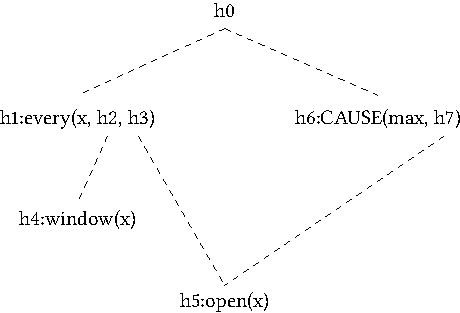
\includegraphics{Figures/max-alle-fenster-oeffnete-mrs-cropped.pdf}
\caption{Max alle Fenster öffnete的支配图\label{Abbildung-Max-alle-Fenster-oeffnete}}
%\caption{Dominance graph for \emph{Max alle Fenster öffnete}\label{Abbildung-Max-alle-Fenster-oeffnete}}
\end{figure}%
图\ref{Abbildung-Max-alle-Fenster-oeffnete}中的每个关系都有一个名词,可以用于指称关系或“抓住”它。这些名词被称作手柄(handle)。这个统制图表明$h0$统制$h1$和$h6$,$h2$统制$h4$,$h3$统制$h5$,$h7$ 统制$h5$。具体的辖域关系不完全赋值:全称量词可以管辖CAUSE,CAUSE也可以管辖全称量词。图\ref{fig-alle-cause}和图\ref{fig-cause-alle}描述了辖域值确定的两个变体。
%Each relation in Figure~\ref{Abbildung-Max-alle-Fenster-oeffnete} has a name that one can use to refer to the relation or ``grasp'' it.
%These names are referred to as \emph{handle}. The dominance graph states that $h0$ dominates both $h1$ and $h6$ and that
%$h2$ dominates $h4$, $h3$ dominates $h5$, and $h7$ dominates $h5$. The exact s\textsc{cop}al relations are underspecified: the universal quantifier can have s\textsc{cop}e over
%CAUSE or CAUSE can have s\textsc{cop}e over the universal quantifier. Figures~\ref{fig-alle-cause} and
%\ref{fig-cause-alle} show the variants of the graph with resolved s\textsc{cop}e.
\begin{figure}
\centering
%% \begin{tabular}{@{}ccc@{}}
%%                                & \mybox[h0]{h0}                & \\[8ex]
%% \mybox[h1]{h1:every(x, \mybox[h2]{h2}, \mybox[h3]{h3})}      &                              & \mybox[h6]{h6:CAUSE(max, \mybox[h7]{h7})}\\[8ex]
%% \mybox[h4]{h4:window(x)}           &         & \\[6ex]
%%                                & \mybox[h5]{h5:open(x)}\\
%% \end{tabular}

%% \begin{tikzpicture}[overlay,remember picture] 
%% \draw(h0.south)--(h1.north); 
%% \draw(h2.south)--(h4.north);
%% \draw(h3.south) .. controls +(0,-1) and +(-1,1)..  (h6.north);
%% \draw(h7.south)--(h5.north);
%% \end{tikzpicture}
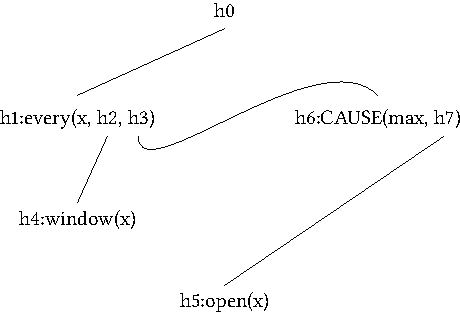
\includegraphics{Figures/solution-mrs-all-cause-open-cropped.pdf}
\caption{$\forall$ x window(x) $\to$ CAUSE(max,open(x))意义的支配图\label{fig-alle-cause}}
%\caption{Dominance graph for the reading $\forall$ x window(x) $\to$ CAUSE(max,open(x)).\label{fig-alle-cause}}
\end{figure}%
\begin{figure}
\centering
%% \begin{tabular}{@{}ccc@{}}
%%                                & \mybox[h0]{h0}                & \\[8ex]
%% \mybox[h1]{h1:every(x, \mybox[h2]{h2}, \mybox[h3]{h3})}      &                              & \mybox[h6]{h6:CAUSE(max, \mybox[h7]{h7})}\\[8ex]
%% \mybox[h4]{h4:window(x)}           &          & \\[6ex]
%%                                & \mybox[h5]{h5:open(x)}\\
%% \end{tabular}

%% \begin{tikzpicture}[overlay,remember picture] 
%% \draw(h0.south)--(h6.north); 
%% \draw(h7.south) .. controls +(0,-1) and +(-1,1)..  (h1.north);
%% \draw(h2.south)--(h4.north);
%% \draw(h3.south)--(h5.north);
%% \end{tikzpicture}
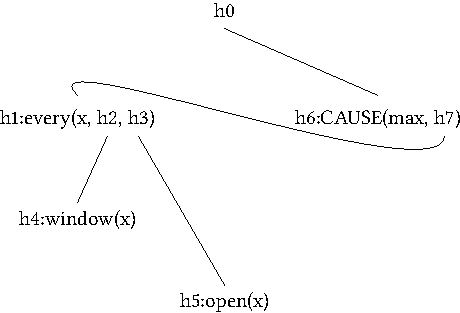
\includegraphics{Figures/solution-mrs-cause-all-open-cropped.pdf}
\caption{CAUSE(max, $\forall$ x window(x) $\to$ open(x))意义的支配图\label{fig-cause-alle}}
%\caption{Graph for te reading CAUSE(max, $\forall$ x window(x) $\to$ open(x)).\label{fig-cause-alle}}
\end{figure}%
图\ref{Abbildung-Max-alle-Fenster-oeffnete}中的不完全赋值图没有说明$h3$和$h6$之间的关系。它显示的唯一信息是:$h3$以某种方式统制$h5$ 。在图\ref{fig-alle-cause}中,每一个($h3$)统制CAUSE ($h6$) ,CAUSE统制open($h5$) 。所以,\relation{every}间接统制\relation{open}。在图\ref{fig-cause-alle}中,CAUSE统制\relation{every},并且\relation{every}统制\relation{open}。图\ref{Abbildung-Max-alle-Fenster-oeffnete}再一次说明了限制,但是$h7$只是间接统制$h5$。
%The underspecified graph in Figure~\ref{Abbildung-Max-alle-Fenster-oeffnete} does not say anything
%about the relation between $h3$ and $h6$. The only thing it says is that $h3$ somehow has to dominate
%$h5$. In Figure~\ref{fig-alle-cause} every ($h3$) dominates CAUSE ($h6$) and CAUSE dominates open
%($h5$). So, \relation{every} dominates \relation{open} indirectly. In Figure~\ref{fig-cause-alle}, CAUSE
%dominates \relation{every} and \relation{every} dominates \relation{open}. Again the constraints of
%Figure~\ref{Abbildung-Max-alle-Fenster-oeffnete} are fulfilled, but $h7$ dominates $h5$ only indirectly.

量词统制$h4$这个事实由量词的词项决定。量词统制$h5$在分析中不用详细地说明,因为量词在属于$h5$的关系中约束一个变量,即x。$h7$和$h5$之间的统制关系在词库中就决定了,因为CAUSE和\relation{open}都只有单独的词项。
%The fact that the quantifier dominates $h4$ is determined by the lexical entry of the quantifier. The fact that
%the quantifier dominates $h5$ does not have to be made explicit in the analysis since the quantifier binds a variable
%in the relation belonging to $h5$, namely x. The dominance relation between $h7$ and $h5$ is always determined in the lexicon
%since CAUSE and \relation{open}  both belong to the semantic contribution of a single lexical entry.

这个分析到底具体采用什么句法理论并不是很重要。这里我们选择HPSG理论。正如图\vref{Abbildung-Fenster-oeffnete-MRS}所示,alle Fenster öffnet的分析包括一个带有动词和宾语的简单结构。
%The exact syntactic theory that one adopts for this analysis is, in the end, not of great importance.
%I have chosen HPSG here. As Figure~\vref{Abbildung-Fenster-oeffnete-MRS} shows, the analysis of \emph{alle Fenster öffnet}
%contains a simple structure with a verb and an object.
\begin{figure}
%\begin{sideways}
\oneline{%
\begin{forest}
sm edges, for tree={l sep= 4ex}
[V$'$\feattab{
    \subcat \sliste{ NP\ind{y} },\\
    \rels \relliste{ h1:every(x, h2, h3), h4:window(x), h6:CAUSE(y,h7), h5:open(x) },\\
    \hcons \relliste{ h0 \qeq h1, h2 \qeq h4, h0 \qeq h6, h7 \qeq h5 }    }
  [\ibox{2} NP\ind{x}\feattab{
    \rels \relliste{ h1:every(x, h2, h3), h4:window(x) },\\
    \hcons \relliste{ h0 \qeq h1, h2 \qeq h4 } } 
    [Det\feattab{
    \rels \relliste{ h1:every(x, h2, h3) },\\
    \hcons \relliste{ h0 \qeq h1, h2 \qeq h4  } } [alle;所有] ]
    [N\feattab{
    \rels \relliste{ h4:window(x) },\\
    \hcons \relliste{ } } [Fenster;窗户] ] ]
  [V\feattab{
                                           \subcat \sliste{ NP\ind{y}, \ibox{2} },\\
                                           \rels \relliste{ h6:CAUSE(y,h7), h5:open(x) },\\
                                           \hcons \relliste{ h0 \qeq h6, h7 \qeq h5 } } [öffnete;打开] ]
]
\end{forest}
}
%\end{sideways}
\caption{\label{Abbildung-Fenster-oeffnete-MRS}alle Fenster öffnete的MRS分析}
%\caption{\label{Abbildung-Fenster-oeffnete-MRS}MRS analysis of \emph{alle Fenster öffnete}}
\end{figure}%
这个结构与alle Kinder kennt (所有儿童都知道)所假设的结构并无明显差异,它包括了语义上单一的动词kennen(知道)。唯一的差异在于所包含的具体动词。正如\ref{Abschnitt-HPSG-Semantik}所示,词之间的关系向上传递。辖域限制也是如此。这些信息都在列表中进行表征。\hcons 代表手柄约束(handle constraints)。h0 \qeq h6中的 \qeq 代表模(modulo)数量词辖域相同。
%This structure does not differ from the one that would be assumed for \emph{alle Kinder kennt} `all
%children know', involving the semantically simplex verb \emph{kennen} `to know'.
%The only difference comes from the meaning of the individual words involved.
%As shown in Section~\ref{Abschnitt-HPSG-Semantik}, relations between individual words are passed on upwards.
%The same happens with s\textsc{cop}al restrictions. These are also represented in lists. \hcons stands for \emph{handle constraints}.
%\qeq in h0 \qeq h6 stand for the equality \emph{modulo} quantifier s\textsc{cop}e.

Egg为例 (\ref{ex-wieder-alle}) 中的句子列出了以下意义⸺重写在 (\mex{1})中:
%Egg lists the following readings for the sentence in (\ref{ex-wieder-alle}) -- repeated here as (\mex{1}):
\ea
\label{ex-wieder-alle-zwei}
\gll dass Max wieder alle Fenster öffnete\\
	 \textsc{comp} Max 再次 所有 窗户 打开\\
\mytrans{Max再次打开了所有这些窗户}
%\gll dass Max wieder alle Fenster öffnete\\
%	 that Max again all windows opened\\
%\mytrans{that Max opened all the windows again}
\z
\begin{enumerate}
\item Max打开了每扇窗户,并且他已经对每扇窗户都至少都打开了一次 (\relation{again}($\forall$(CAUSE(open)));重复性)
%\item Max opened every window and he had already done that at least once for each window
%      (\relation{again}($\forall$(CAUSE(open))); repetitive)
\item Max致使每扇窗户都开了,并且他已经对每扇窗户都打开了一次 (\relation{again}(CAUSE($\forall$(open)));重复性)
%\item Max caused every window to be open and he had done that at least once before 
%      (\relation{again}(CAUSE($\forall$(open))); repetitive)
\item 在更早的某一个时间,所有的窗户同时开着,并且Max将所有的窗户恢复到开着的状态(CAUSE(\relation{again}($\forall$(open))); 恢复性)
%\item At some earlier point in time, all windows were simultaneously open and Max re-established this state
%      (CAUSE(\relation{again}($\forall$(open))); restitutive)
\end{enumerate}

\noindent
这些意义对应于图\vref{Abbildung-Max-wieder-alle-Fenster-oeffnete}中支配图的意义。
%These readings correspond to the dominance graph in Figure~\vref{Abbildung-Max-wieder-alle-Fenster-oeffnete}.
\begin{figure}
\centering
%%   \begin{tabular}{@{}ccc@{}}
%%   & \mybox[h0]{h0}                       & \\[4ex]
%%     \mybox[h8]{h8:again}\mybox[h9]{(h9)}  \\[4ex]
%%     \mybox[h1]{h1:every(x, \mybox[h2]{h2}, \mybox[h3]{h3})}      &                              & \mybox[h6]{h6:CAUSE(max, \mybox[h7]{h7})}\\[8ex]
%%   \mybox[h4]{h4:window(x)}           &          & \\[6ex]
%%                            & \mybox[h5]{h5:open(x)}\\
%%   \end{tabular}

%% \begin{tikzpicture}[overlay,remember picture,dashed] 
%% \draw(h0.south)--(h8.north); 
%% \draw(h0.south)--(h6.north);
%% \draw(h9.south)--(h1.north);
%% \draw(h2.south)--(h4.north);
%% \draw(h3.south)--(h5.north);
%% \draw(h7.south)--(h5.north);
%% \end{tikzpicture}
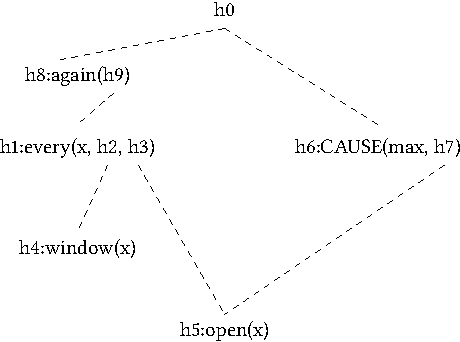
\includegraphics{Figures/mrs-max-wieder-alle-fenster-oeffnete-cropped.pdf}
\caption{Max wieder alle Fenster öffnete(Max再次打开了所有这些窗户)\label{Abbildung-Max-wieder-alle-Fenster-oeffnete}的支配图}
%\caption{Dominance graph for \emph{Max wieder alle Fenster öffnete} `that Max opened all the
%  windows again'\label{Abbildung-Max-wieder-alle-Fenster-oeffnete}}
\end{figure}%
图\vref{Abbildung-Max-alle-Fenster-wieder-oeffnete} 展示了 (\ref{ex-alle-wieder})的图⸺重写为(\mex{1}):
%Figure~\vref{Abbildung-Max-alle-Fenster-wieder-oeffnete} shows the graph for (\ref{ex-alle-wieder})
%-- repeated here as (\mex{1}):\todostefan{Skopus hinzufügen?}
\addlines
\ea
\label{ex-alle-wieder-zwei}
\gll dass Max alle Fenster wieder öffnete\\
	 \textsc{comp} Max 所有 窗户 再次 打开\\
%\gll dass Max alle Fenster wieder öffnete\\
%	 that Max all windows again opened\\
\mytrans{Max再次打开所有的窗户}
\z
\begin{figure}
\centering
%% \begin{tabular}{@{}ccc@{}}
%%                                & \mybox[h0]{h0}                & \\[8ex]
%% \mybox[h1]{h1:every(x, \mybox[h2]{h2}, \mybox[h3]{h3})}      &                              &                               \mybox[h6]{h6:CAUSE(max, \mybox[h7]{h7})}\\[4ex]
%%                                                               \multicolumn{2}{c}{\hspace{3em}\mybox[h8]{h8:again(\mybox[h9]{h9})}}\\[4ex]
%% \mybox[h4]{h4:window(x)}           &          & \\[6ex]
%%                                & \mybox[h5]{h5:open(x)}\\
%% \end{tabular}
%% \begin{tikzpicture}[overlay,remember picture,dashed] 
%% \draw(h0.south)--(h1.north); 
%% \draw(h0.south)--(h6.north);
%% \draw(h2.south)--(h4.north);
%% \draw(h3.south)--(h8.north);
%% \draw(h9.south)--(h5.north);
%% \draw(h7.south)--(h5.north);
%% \end{tikzpicture}
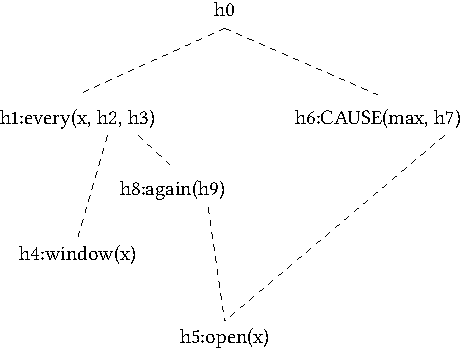
\includegraphics{Figures/mrs-max-alle-fenster-wieder-oeffnete-cropped.pdf}
\caption{Max alle Fenster wieder öffnete(Max再次打开所有这些窗户)的支配图\label{Abbildung-Max-alle-Fenster-wieder-oeffnete}}
%\caption{Dominance graph for \emph{Max alle Fenster wieder öffnete} `that Max opened all the
%  windows again'\label{Abbildung-Max-alle-Fenster-wieder-oeffnete}}
\end{figure}%
从这些没有wieder(再次)的例句中推导出这些统制图,需要做的只是增加表达式h8:again(h9)和支配要求,要求$h9$统制出现在wieder右边的量词,要求h9被wieder左边的量词统制。
%To derive these dominance graphs from the ones without \emph{wieder} `again', all one has to do is add the expression h8:again(h9)
%and the dominance requirements that demand that $h9$ dominates quantifiers occurring to the right of \emph{wieder} and that it
%is dominated by quantifiers to the left of \emph{wieder}.

所以在不借助为CAUSE和BECOME设置空语类的前提下,就可以很轻易地推导出wieder所修饰的相关意义。词语öffnen的意义以相似的方式分解,但是被分解的意义被指派到一个单独的成分上,即动词。通过在词库中不完全赋值的辖域关系,相关意义都可以推导出来。
%It is therefore unproblematic to derive the relevant readings for modification by \emph{wieder}
%without empty elements for CAUSE and BECOME. The meaning of the word \emph{öffnen} is decomposed in a similar way but the
%decomposed meaning is assigned to a single element, the verb. By underspecification of the s\textsc{cop}al
%relations in the lexicon, the relevant readings can then be derived. 


%% Shravan sagt nee, wahrscheinlich nicht. 24.06.2008
%% Unterspezifikation ist auch psycholinguistisch plausibler als die explizite Ableitung aller Skopus:
%% Es ist unwahrscheinlich, dass Menschen für normale Sätze jeweils Tausende Repräsentationen
%% verwenden, die sich nur in verschiedenen Skopus unterscheiden. Stattdessen lassen sie wahrscheinlich
%% die Bedeutung weitestgehend unterspezifiziert und lösen sie dann bei ausreichendem Kontextwissen
%% weiter auf.

\section{空语类的证据}
%\section{Evidence for empty elements}
\label{Abschnitt-Evidenz-leere-Elemente}

正如前面所讨论的,语法学家认为语言学家和说话者都能注意到一个词串中什么时候会缺少一个成分。对于那些是否存在语迹,凭经验无法区分的现象,可以假设存在空语类。但是,构式语法学家提出的学习能力的论据还是有些说服力的:如果假设没有天赋语言学知识或者天赋语言学知识很少的话,那么就不能用来自其他语言的语料来证明空语类的存在。正如 \citet{Stechow96a}和 \citet{Meinunger2000a}所做的那样,巴斯克语\ilce{巴斯克语}{Basque}有宾语一致性\iscesub{一致关系}{agreement}{宾语}{object}的问题;并不意味着可以在德语语法中为宾语的一致(AgrO\iscesubsub{范畴}{category}{功能}{functional}{AgrO}{AgrO})假设一个空的中心语。因为德语中没有宾语一致性的问题,儿童不可能学到有一个AgrO中心语这样的事实。因此,关于AgrO的知识必须是天赋的。因为天赋知识的假设存在争议(见第\ref{chap-innateness}章),任何使用跨语言现象来支持使用空语类的理论,其基础都是不稳固的。
%As previously discussed, grammarians agree that both linguists and speakers notice when there is a constituent missing from a
%string of words. For cases where it can be shown that analyses with or without traces are indistinguishable empirically,
%then one can assume empty elements. Nevertheless, the learnability argument put forward by
%Construction Grammarians has some validity: if one assumes that there is no or little innate linguistic knowledge, then it is not possible to motivate empty elements
%with data from other languages. This means that just because Basque\il{Basque} shows object agreement\is{agreement!object},
%this does not mean that one can assume an empty head for object agreement
%(AgrO\is{category!functional!AgrO}) in a grammar of German as
%for instance  \citet{Stechow96a} and  \citet{Meinunger2000a} do. Since there is no object agreement in German, there
%would be no way for the child to learn the fact that there is an AgrO head. Knowledge about AgrO
%must therefore be innate. Since the assumption of innate linguistic knowledge is controversial (see
%Chapter~\ref{chap-innateness}), any theory that uses cross-linguistic data to motivate the use of empty elements is on shaky ground.

只有在多种分析方法之间没有实际差异,并且受到当前研究的语言的启示时,才能参照跨语言的现象进行分析。在这一点上,应该遵循奥卡姆剃刀原则,选择与其他语言分析兼容的分析(见\citealp{MuellerCoreGram}和第\ref{sec-develop-theories-coregram}章)。
\isce[|)]{空成分}{empty element}
%Cross-linguistic considerations can only be drawn upon if there are no empirical differences between multiple alternative
%analyses compatible and motivated by the language under consideration. In this case, one should follow Occam's Razor and choose the analysis which is compatible with analyses of
%other languages (see \citealp{MuellerCoreGram} and Chapter~\ref{sec-develop-theories-coregram}).
%\is{empty element|)}

\section{转换,词汇规则和空语类}
%\section{Transformations, lexical rules, and empty elements}
\label{Abschnitt-leere-Elemente-LRs-Transformations}

在\isce[|(]{空成分}{empty element}\isce[|(]{词汇规则}{lexical rule}\isce[|(]{转换}{transformation}TAG框架内对被动式\isce{被动}{passive}的讨论中,我们已经清楚的是词汇规则对应特定的转换式,即那些与一个词项有关的转换式(词汇管辖的转换式,\citet{Dowty78a};关于转换式和词汇规则的讨论,可以参见 \citew{Bresnan78a}和 \citew{BK82a})。在TAG\indextag 各自的变体中,词汇规则在一个词项的主动句法树和被动句法树之间建立联系。主动句法树和被动句法树都可以通过附加进行扩展。
%In\is{empty element|(}\is{lexical rule|(}\is{transformation|(} the discussion of the passive\is{passive} in the framework of TAG, it became clear that lexical rules
%correspond to particular transformations, namely those which have some relation to a lexical item (lexically governed transformations, \citealp{Dowty78a}; 
%for the discussion of transformations and lexical rules, see  \citew{Bresnan78a} and  \citew{BK82a}). In the respective variants of TAG\indextag, lexical rules establish a relation
%between a lexical item for an active tree with a lexical item of a passive tree. Both the active and passive tree can be extended by adjunction.

在范畴语法\indexcg 等理论中,情况是一样的:因为一个功能符寻找其论元的方向在英语这样的语言中是固定的,所以词项代表整棵句法树。附加语不需要在词项中进行说明。附加语可以出现在句法树的什么位置取决于附加语的属性。在\ref{Abschnitt-CG-lokale-Umstellung}中,我们已经看到如何处理语序自由的语言。如果组合的方向没有在词库中确定,那么词项就可以出现在多个句法树中。如果我们对比用于这类词项的词汇规则和转换,也能够看到在不同句法树集合中产生关系的词汇规则。
%In theories such as Categorial Grammar\indexcg, the situation is similar: since the direction in which a functor expects to find its argument is fixed
%for languages such as English, the lexical item stands for an entire tree. Only the attachment of
%adjuncts is not yet specified in lexical items. The positions in the
%tree where the adjuncts can occur depend on the properties of the adjuncts. In Section~\ref{Abschnitt-CG-lokale-Umstellung},
%we have seen suggestions for treatments of languages with free constituent order. If the direction of combination is not fixed in the lexicon, then the lexical item
%can occur in a number of trees. If we compare lexical rules that can be applied to this kind of lexical items with transformations, we see that lexical rules create relations
%between different sets of trees.

在\hpsgc 分析\indexhpsg 中,方式也很相似:词汇规则将价属性不同的词项互相联系起来。在英语\ilce{英语}{English}的HPSG语法中,通常有一个模式允准一个VP,该VP包括动词及其所有补足语;还有一个模式将主语和这一VP连接起来\citep[\page 39]{ps2}。在定式动词的词项中,已经确定了句法树最后的样子。与在范畴语法中一样,HPSG中的附加语可以与多种中间投射组合。基于在特定语法中使用的统制模式,词项会决定能够出现的成分结构和允许出现的多重结构。在第\ref{Kapitel-HPSG}章提出的德语语法中,可以使用双及物动词的词项来分析六种不同的序列,即,在六种动词居末的结构中,词项都可以不考虑附加语。两种序列可以用被动词项来分析,该词项只有两个论元。正如在范畴语法中分析的一样,被允准结构的集合与其他被允准结构的集合相互联系。在HPSG理论和构式语法中,曾努力用其他机制来代替词汇规则,因为词汇规则“地位是含糊的,并且与其他分析的互动是存在争议的”\citep*[\page 19]{BMS2001a}。 \citet{BMS2001a} 提出了一种分析方法:不是将具有不同价列表的词项连接起来,而是在同一个词项中一个列表的次集合和另外一个列表之间建立联系。两种分析方法的结果分别见(\mex{1})和(\mex{2}):
%In \hpsg analyses\indexhpsg, this works in a similar way: lexical rules relate lexical items with differing valence properties to each other. In HPSG grammars of English\il{English},
%there is normally a schema that licenses a VP containing the verb and all its complements as well as a schema that connects the subject to the VP 
%\citep[\page 39]{ps2}. In the lexical items for finite verbs, it is already determined what the tree will look like in the end. As in Categorial Grammar, adjuncts in HPSG can
%be combined with various intermediate projections. Depending on the dominance schemata used in a particular grammar, the lexical item will determine the constituent structure
%in which it can occur or allow for multiple structures. In the grammar of German proposed in Chapter~\ref{Kapitel-HPSG}, it is possible to analyze six different sequences with a lexical
%item for a ditransitive verb, that is, the lexical item can -- putting adjuncts aside -- occur in six different structures with verb-final order. Two sequences can be analyzed
%with the passive lexical item, which only has two arguments.
%As in Categorial Grammar, sets of licensed structures are related to other sets of licensed structures. In HPSG theorizing and also in Construction Grammar, there have been
%attempts to replace lexical rules with other mechanisms since their ``status is dubious and their interaction with other analyses is controversial''
%\citep*[\page 19]{BMS2001a}.  \citet{BMS2001a} propose an analysis for extraction
%that, rather than connecting lexical items with differing valence lists, establishes a relation between a subset of a particular list in a lexical item and another
%list in the same lexical item. The results of the two alternative analyses are shown in (\mex{1})
%and (\mex{2}), respectively:
\eal
\ex \ms{ subcat & \sliste{ NP[\type{nom}], NP[\type{acc}] }\\
         slash  & \eliste\\
       }
\ex \ms{ subcat & \sliste{ NP[\type{nom}] }\\
         slash  & \sliste{ NP[\type{acc}] }\\
       }
\zl
在(\mex{0})中,(\mex{0}a)是一个基本词项,而(\mex{0}b)通过一个词汇规则与 (\mex{0}a)联系。另一种分析只是说明了\textsc{arg-st}特征\isfeat{arg-st}的合适取值\footnote{%
\argstc 代表论元结构。\argstc 的取值是一个列表,包含一个中心语的所有论元。关于\argstc 更多的信息,可以参见\ref{Abschnitt-Arg-St}。
},而\subcatc 和\slashvc 都是通过相关限制从\argstvc 推导而来的。(\mex{1})显示了两个被允准的词项。
%In (\mex{0}), (\mex{0}a) is the basic entry and (\mex{0}b) is related to (\mex{0}a) via a lexical
%rule. The alternative analysis would only involve specifying the appropriate value
%of the \textsc{arg-st} feature\footnote{%
%\argst stands for \emph{Argument Structure}. The value of \argst is a list containing all the arguments
%of a head. For more on \argst, see Section~\ref{Abschnitt-Arg-St}.
%}\isfeat{arg-st} and the \subcat and \slashv is then derived from the \argstv using the relevant constraints.
%(\mex{1}) shows two of the licensed lexical items.
\eal
\ex \ms{ arg-st & \sliste{ NP[\type{nom}], NP[\type{acc}] }\\
         subcat & \sliste{ NP[\type{nom}], NP[\type{acc}] }\\
         slash  & \eliste\\
       }
\ex \ms{ arg-st & \sliste{ NP[\type{nom}], NP[\type{acc}] }\\
         subcat & \sliste{ NP[\type{nom}] }\\
         slash  & \sliste{ NP[\type{acc}] }\\
       }
\zl
如果我们想以这种方式完全取消词汇规则,那么我们需要为每一种变化设置额外的特征。 \footnote{%
换一种方式,可以假设一个非常复杂的关系来联系\argstc 和\subcatc。但是这必须带来一系列现象互动的结果,并且这些现象的互动无法用一种明显的方式表征。%
} 因为有很多交互的变价过程,所以需要标明很多助动词特征。这种分析的结果在 \citew[第7.5.2.2节]{MuellerLehrbuch1}中已经详细讨论过了。这里产生的问题与基于承继的方法解决论元结构变化过程遇到的问题一样:这种分析也需要助动词特征,因为不可能用承继来刻画论元信息的嵌套和多重改变。见\ref{Abschnitt-Passiv-CxG}。
%If we want to eliminate lexical rules entirely in this way, then we would require an additional feature for each change.\footnote{%
%Alternatively, one could assume a very complex relation that connects \argst and \subcat. But this would then have to deliver
%the result of an interaction of a number of phenomena and the interaction of these phenomena would not be captured in a transparent way.%
%} Since there are many interacting valence-changing processes, things only work out with the stipulation of a large number of auxiliary
%features. The consequences of assuming such analyses have been discussed in detail in
% \citew[Section~7.5.2.2]{MuellerLehrbuch1}. The problems that arise are parallel for
%inheritance-based approaches for argument structure-changing processes: they also require
%auxiliary features since it is not possible to model embedding and multiple changes of valence information with inheritance. See Section~\ref{Abschnitt-Passiv-CxG}.

另外,词汇规则的地位很模糊这个观点也应该遭到反对:因为存在很多成型的词汇规则形式化体系\citep{Meurers2001a,CB92a,LC99a},并且它们与其他分析的互动也不存在争议。大多数HPSG装置都使用词汇规则,并且大量词汇规则和约束可以试着用语法片段来确认。
%Furthermore, the claim that the status of lexical rules is dubious must be rejected: there are worked-out formalizations of lexical rules \citep{Meurers2001a,CB92a,LC99a}
%and their interaction with other analyses is not controversial. Most HPSG implementations make use of lexical rules and the interaction of a number of rules and
%constraints can be easily verified by experiments with implemented fragments.

 \citet{Jackendoff75a}给出了词汇规则的两个可能的概念:在一个概念中,词库包含一个给定语言中的所有词,并且只有冗余规则来说明词项的一些属性与另外一些词项的属性如何表现。例如,les(读)和lesbar(可读的)在词库中有相同的地位。词汇规则的另外一个概念是,有一些基本词项,并且其余的词项是借助词汇规则从这些基本词项推导出来的。词干les是基本词项,并且lesbar是从它推导出来的。在HPSG中,常常使用第二种定义。这等同于单分支规则假设。在第\pageref{Abbildung-Verbstellung-HPSG}页的图\ref{Abbildung-Verbstellung-HPSG},就是如此展示的:动词kennt(知道)通过一个词汇规则映射到一个动词,该动词选择一个空的动词中心语进行投射。借助词汇规则,可以通过假设有一个含有空的中心语的二叉结构而不是单分支规则来把词汇规则从语法中清除出去。例如,在HPSG对于动结构式\isce{动结构式}{resultative construction}\iscesub[|(]{构式}{construction}{动结}{resultative}的分析中,如(\mex{1})就提出了词汇规则 (\citealp{Verspoor97a};\citealp{Wechsler97a};\citealp{WN2001a};\citealp[第5章]{Mueller2002b})。
% \citet{Jackendoff75a} presents two possible conceptions of lexical rules: in one variant, the lexicon contains all words in a given language and there
%are just redundancy rules saying something about how certain properties of lexical entries behave with regard to properties of other lexical entries. For example,  \stem{les} `read-' and \emph{lesbar}
%`readable' would both have equal status in the lexicon. In the other way of thinking of lexical
%rules, there are a few basic lexical entries and the others are derived
%from these using lexical rules. The stem  \stem{les} `read-' would be the basic entry and \emph{lesbar} would be derived from it.
%In HPSG, the second of the two variants is more often assumed. This is equivalent to the assumption of unary rules. In Figure~\ref{Abbildung-Verbstellung-HPSG} on
%page~\pageref{Abbildung-Verbstellung-HPSG}, this has been shown accordingly: the verb \emph{kennt}
%`knows' is mapped by a lexical rule to a verb that selects the projection of an
%empty verbal head. With this conception of lexical rules, it is possible to remove lexical rules from the grammar by assuming binary-branching structures with an
%empty head rather than unary rules. For example, in HPSG analyses of resultative constructions\is{resultative construction}\is{construction!resultative|(}
%such as (\mex{1}), lexical rules have been proposed (\citealp{Verspoor97a}; \citealp{Wechsler97a}; \citealp{WN2001a}; \citealp[Chapter~5]{Mueller2002b}).
\ea
\gll [dass] Peter den Teich leer fischt\\
	 \spacebr{}\textsc{comp} Peter \defart{} 池塘 空 钓\\
\mytrans{Peter钓空了池塘}
%\gll [dass] Peter den Teich leer fischt\\
%	 \spacebr{}that Peter the pond empty fishes\\
%\mytrans{that Peter fishes the pond empty}
\z
在我们的分析中,词汇规则将一个不及物动词跟一个动词连接起来,该动词选择一个宾格宾语和另一个谓词。图\vref{Abbildung-Resultativ-LR}展示了对应的句法树。
%In my own analysis, a lexical rule connects a verb used intransitively to a verb that selects an accusative object and a predicate.
%Figure~\vref{Abbildung-Resultativ-LR} shows the corresponding tree.
\begin{figure}
\centering
\begin{forest}
sm edges
[V{[\subcat \eliste]}
	[NP{[\type{nom}]}
		[Peter;Peter]]
	[V{[\subcat \sliste{ NP[\type{nom}] }]}
		[NP{[\type{acc}]}
			[den Teich;\textsc{da} 池塘, roof]]
		[V{[\subcat \sliste{ NP[\type{nom}], NP[\type{acc}] } ]}
			[Adj
				[leer;空]]
			[V{[\subcat \sliste{ NP[\type{nom}], NP[\type{acc}], Adj } ]}
				[V{[\subcat \sliste{ NP[\type{nom}]} ]}
					[fischt;钓]]]]]]
\end{forest}
\caption{\label{Abbildung-Resultativ-LR}使用词汇规则对动结构式进行的分析}
%\caption{\label{Abbildung-Resultativ-LR}Analysis of the resultative construction with a lexical rule}
\end{figure}%
如果我们考虑一下(\mex{0}) 的意思,就可以发现钓鱼行为导致鱼塘变空了。这个致使关系没有包括在(\mex{0})中词语的任意一个词项中。为了让这个信息出现在整个表达式的语义表示中,必须通过词汇规则来添加这个信息。词汇规则规定:如果一个动词选择限制另一个谓词和受格宾语,那么整个构式具有一种致使意义。
%If we consider what (\mex{0}) means, then we notice that the fishing act causes the pond to become empty.
%This causation is not contained in any of the basic lexical items for the words in (\mex{0}).
%In order for this information to be present in the semantic representation of the entire expression, it has
%to be added by means of a lexical rule. The lexical rule says: if a verb is used with an additional predicate and accusative
%object, then the entire construction has a causative meaning.

图\vref{Abbildung-Resultativ-leer}展示了怎样用一个空的中心语替代一个词汇规则。
%Figure~\vref{Abbildung-Resultativ-leer} shows how a lexical rule can be replaced by an empty head.
\begin{sidewaysfigure}
\centering
%\scalebox{0.9}{%
\begin{forest}
sm edges
[V{[\subcat \eliste]}
	[{NP[\type{nom}]}
		[Peter;Peter]]
	[{V[\subcat \sliste{ NP[\type{nom}] }]}
		[{NP[\type{acc}]}
			[den Teich;\textsc{da} 池塘,roof]]
		[{V[\subcat \sliste{ NP{[\type{nom}]}, NP{[\type{acc}]} }]}
			[Adj
				[leer;空]]
			[{[\subcat \sliste{ NP{[\type{nom}]}, NP{[\type{acc}]}, Adj }]}
				[{V[\subcat \sliste{ NP{[\type{nom}]} }]}
					[fischt;钓]]
				[{V[\subcat \sliste{ NP{[\type{nom}]}, NP{[\type{acc}]}, Adj, V{[\subcat \sliste{ NP{[\type{nom}]} }]} }]}
					[\trace]]]]]]
\end{forest}
%}
\caption{\label{Abbildung-Resultativ-leer}使用空中心语对动结构式进行的分析}
%\caption{\label{Abbildung-Resultativ-leer}Analysis of the resultative construction with an empty head}
\end{sidewaysfigure}%
空的中心语需要一个不及物动词、一个形容词、一个受格宾语和一个主语。Fischt(钓鱼)的主语当然要与空中心语的主语一致。这一点没有呈现在图中。但是,可以建立这一等同性(参见\citealp{HN94a})。在这个分析中,致使语义是由空的中心语贡献的。这里使用的技巧正是在\ref{Abschnitt-Eleminierung-leerer-Elemente}中所使用的,只是方向相反:在前面的章节中,含有空的子结点的二叉结构被单分支结构所替代。在这一节中,我们用含有空的子结点的二叉结构代替单分支结构。\dotfootnote{%
这里,我们讨论词汇规则,但是这个转换技巧也可以运用到其他单分支规则上。语义学家经常用这种规则来完成类型转换\isce{类型提升}{type raising}。例如,一个规则将一个指称性NP(例如,i.a中的a trickster)转变为一个谓词性成分(i.b)\citep{Partee87a-u}。
\eal
\ex 
\gll A trickster laughs.\\
一 骗子 大笑\\
\mytrans{骗子在大笑。}
\ex 
\gll He is a trickster.\\
他 \textsc{cop} 一 骗\\
\mytrans{他是个骗子。}
\zl
这些转变可以通过作用于一个NP的单分支规则或者一个以NP作为其论元的特殊的空的中心语完成。在现在的最简方案\indexmp 中,使用空的中心语\citep[\page 370]{Ramchand2005a},而在范畴语法\indexcg 和HPSG\indexhpsg 中使用单分支规则更为常见 (\citealp[\page 91--92]{Flickinger2008a};\citealp{MuellerPredication,MuellerCopula})。
}\isce[|)]{空成分}{empty element}\isce[|)]{词汇规则}{lexical rule}\isce[|)]{转换}{transformation}\iscesub[|)]{构式}{construction}{动结}{resultative}
%The empty head requires the intransitive verb and additionally an adjective, an accusative object and a subject.
%The subject of \emph{fischt} `fishes' must of course be identical to the subject that is selected by the combination
%of \emph{fischt} and the empty head. This is not shown in the figure.
%It is possible, however, to establish this identity (see \citealp{HN94a}). The causative semantics is contributed by
%the empty head in this analysis. The trick that is being implemented here is exactly what was done in Section~\ref{Abschnitt-Eleminierung-leerer-Elemente},
%just in the opposite direction: in the previous section, binary-branching structures with an empty daughter were replaced by unary-branching structures.
%In this section, we have replaced unary-branching structures with binary-branching structures with an empty daughter.\footnote{%
%	Here, we are discussing lexical rules, but this transformation trick can also be applied to
%        other unary rules. Semanticists often use such rules for type shifting\is{type raising}. For
%        example, a rule that turns a referential NP such as \emph{a trickster} in (i.a) into a
%        predicative one (i.b) \citep{Partee87a-u}.
%\eal
%\ex A trickster laughs.
%\ex He is a trickster.
%\zl
%These changes can be achieved by a unary rule that is applied to an NP or with a special empty head that takes an NP as its argument. In current Minimalist\indexmp approaches,
%empty heads are used \citep[\page 370]{Ramchand2005a}, in Categorial Grammar\indexcg and HPSG\indexhpsg unary-branching rules are more common (\citealp[\page
%    91--92]{Flickinger2008a}; \citealp{MuellerPredication,MuellerCopula}).
%}\is{empty element|)}\is{lexical rule|)}\is{transformation|)}\is{construction!resultative|)}

我们已经看到一些转换可以被词汇规则替换,而一些词汇规则可以被空的中心语替换。下面的章节解决以下问题:提取、置换、被动等现象是不是应该像在GB/最简方案中统一描述或者像在LFG和HPSG中用不同的工具描述。
%We have therefore seen that certain transformations can be replaced by lexical rules and also that
%lexical rules can be replaced by empty heads. 
%The following chapter
%will deal with the question of whether meaning is contributed by lexical heads or rather holistically by phrasal configurations.
%deals with the question of whether phenomena like extraction, scrambling, and passive should be
%described with the same tool as in GB/Minimalism or with different tools as in LFG and HPSG.


%      <!-- Local IspellDict: en_US-w_accents -->
